\chapter{Metodologia Proposta}
\label{chap3}

No capítulo anterior, foram apresentados os conceitos e as tecnologias relevantes para a compreensão da solução de monitoramento desenvolvida. Contudo, vale ressaltar que nem todas as ferramentas descritas foram efetivamente empregadas na implementação final da proposta.

Este capítulo tem por objetivo detalhar todo o processo de desenvolvimento da solução de monitoramento, desde as primeiras considerações e escolhas de arquitetura, passando pela seleção e adaptação das ferramentas adotadas, até a apresentação da solução final implementada. Serão discutidas as motivações para determinadas decisões técnicas, desafios encontrados ao longo do desenvolvimento, e os métodos empregados para contorná-los, buscando sempre respaldar as opções feitas com base nos conceitos apresentados no Capítulo 2. Também são descritos os equipamentos utilizados durante o desenvolvimento e todo o código fonte do projeto está versionado no repositório Git \citep{vitorcossetti2025}.

As especificações do sistema operacional serão apresentadas posteriormente, visto que a escolha desse aspecto evoluiu ao longo do desenvolvimento, conforme será detalhado neste capítulo.

\section{Abordagem Preliminar}
\label{section:AbordagemPreliminar}

Esta seção apresenta uma visão geral das decisões iniciais tomadas antes da definição da arquitetura final da solução de monitoramento. As primeiras etapas deste trabalho podem ser divididas em dois momentos: inicialmente, o escopo era voltado para o monitoramento de infraestruturas de TI tradicionais (como servidores e clusters); em seguida, evoluiu para englobar também dispositivos conectados à rede de forma abrangente, sem restrições de tipagem.

\subsection{Escopo inicial - Infraestrutura Tradicional}
\label{subsection:EscopoInicial}

Durante as discussões preliminares, o objetivo era monitorar servidores. Foi considerada uma arquitetura onde um dispositivo --- podendo ser um NUC ou Raspberry Pi com softwares instalados --- realizaria a coleta de métricas deste servidor e, após o processamento destes dados, disponibilizaria-os em painéis com visualizações gráficas especializadas. Alternativas com Orange Pi como equipamento foram analisadas, mas a escolha final recaiu sobre o NUC ou Raspberry Pi devido à suas respectivas popularidades e suporte.

Entretanto, como não foi possível adquirir fisicamente um NUC ou Raspberry Pi, decidiu-se simular toda a \foreign{stack} de monitoramento em uma máquina virtual. Com isso, a possibilidade da utilização de distribuições ou versões do Raspberry Pi OS para fins de desenvolvimento foi descartada, por tratar-se de um sistema operacional baseado em arquitetura ARM, incompatível com a arquitetura x86-64 dos equipamentos disponíveis.

No \foreign{desktop} disponível, à época com sistema operacional não-Linux, instalou-se o VMWare Workstation Player (versão gratuita do VMWare Workstation) para configuração de uma VM com Rocky Linux. A escolha do deste SO\abbrev{SO}{Sistema Operacional} baseou-se em sua compatibilidade com o CentOS, estabilidade e longo ciclo de suporte, características valorizadas em ambientes corporativos.

No entanto, o VMWare Workstation Player mostrou-se limitado em recursos, dificultando a execução de múltiplas VMs. Por isso, migrou-se para o VirtualBox, o que trouxe maior flexibilidade e controle.

Esta estratégia inicial apresentou limitações importantes: a primeira era a maior dificuldade na aquisição de dados, pois seria necessário obter um servidor físico para coleta dos mesmos. Outra limitação foi o elevado custo computacional inerente ao uso de VMs em comparação a soluções baseadas em contêineres, e pouca modularidade, resultando em manutenção complexa e baixa praticidade.

Devido a esses fatores, verificou-se a necessidade de reavaliar o escopo e buscar abordagens mais aderentes aos recursos disponíveis e aos objetivos do projeto.

\begin{figure}[H]
\centering
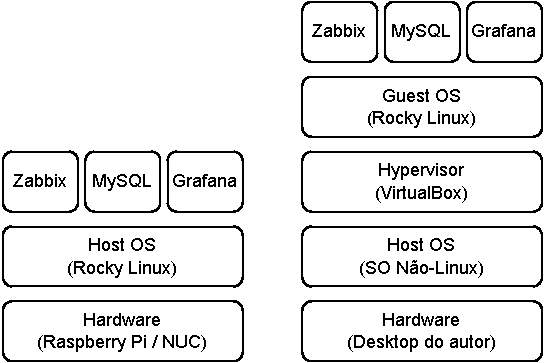
\includegraphics[scale=1]{Imagens/chap03/v0xv1_stack.pdf}
\caption{Da esquerda para a direita - \foreign{stack} conceitual, \foreign{stack} implementada.}
\label{fig:StackImplementada}
\end{figure}

\begin{figure}[H]
\centering
\setlength{\abovecaptionskip}{-20pt}
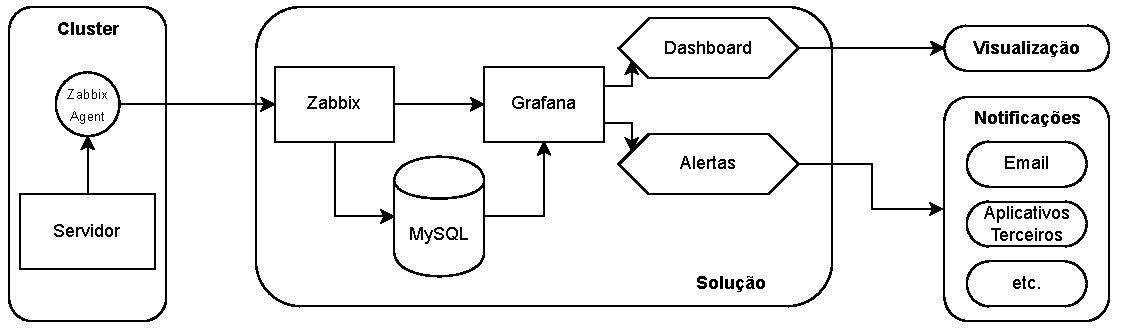
\includegraphics[width=\textwidth]{Imagens/chap03/v0_diagram.pdf}
\caption{Arquitetura conceitual.}
\label{fig:ArquiteturaConceitual}
\end{figure}

\begin{figure}[H]
\centering
\setlength{\abovecaptionskip}{-20pt}
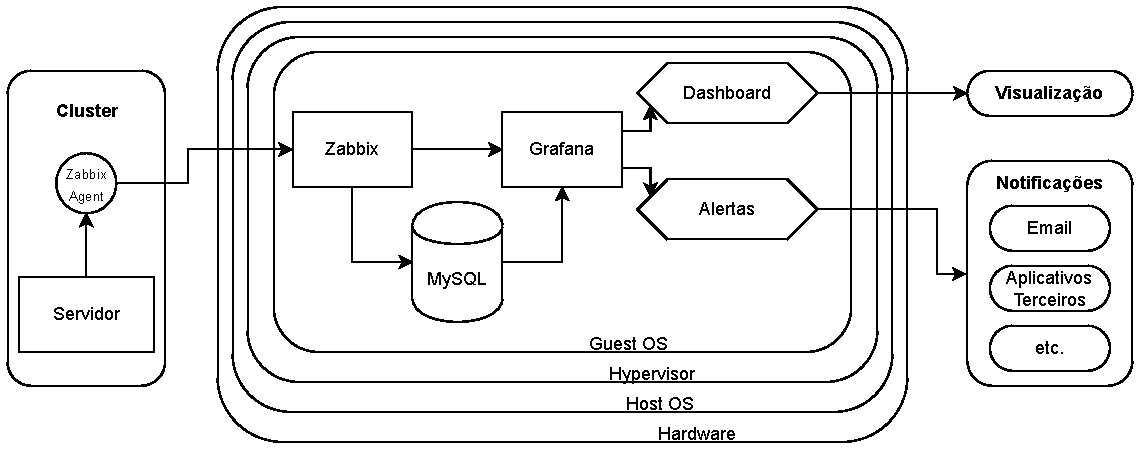
\includegraphics[width=\textwidth]{Imagens/chap03/v1_diagram.pdf}
\caption{Arquitetura implementada.}
\label{fig:ArquiteturaImplementada}
\end{figure}

\subsection{Escopo Reformulado - Monitoramento Amplo}
\label{subsection:EscopoReformulado}

Até então, os sistemas operacionais dos \foreign{hosts} disponíveis eram distintos (o \foreign{desktop} com um sistema não-Linux e o \foreign{notebook} com Ubuntu Desktop). Considerando as limitações encontradas na abordagem inicial, optou-se por instalar o Ubuntu Server no desktop como SO para experimentação.

Conforme relatado na literatura, o Ubuntu Server demonstrou desempenho satisfatório e baixo consumo de recursos. Contudo, havia dois equipamentos sendo utilizados no desenvolvimento do projeto: 1 -- \foreign{desktop} do próprio autor, sem qualquer restrição para troca e alteração de hardware e software; 2 -- \foreign{notebook} corporativo em que o sistema operacional não poderia ser alterado. Visando padronizar os ambientes de desenvolvimento, decidiu-se por padronizar o SO no Ubuntu Desktop em ambos os dispositivos.

No decorrer dessas alterações, a abordagem de monitoramento foi ampliada para contemplar não apenas servidores, mas também uma ampla variedade de dispositivos conectados à rede. Essa redefinição proporcionou maior versatilidade ao projeto, tornando desnecessária a aquisição de servidores físicos e possibilitando a utilização de contêineres tanto para a simulação de dispositivos quanto para a implementação da \foreign{stack} de monitoramento. Com isso, o processo de desenvolvimento tornou-se mais prático, ágil e modular, além de permitir um aproveitamento mais eficiente dos recursos computacionais disponíveis. Cabe destacar ainda que, ao adotar contêineres não só para testes, mas também para toda a infraestrutura de monitoramento, a discussão sobre a necessidade de hardware específico, como NUC ou Raspberry Pi, perdeu relevância neste contexto, já que a solução desenvolvida pode ser executada em qualquer máquina compatível com tecnologias de conteinerização.

\begin{figure}[H]
\centering
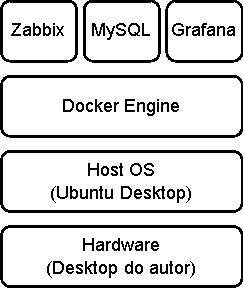
\includegraphics[scale=0.97]{Imagens/chap03/v2_stack.pdf}
\caption{\foreign{Stack} reformulada.}
\label{fig:StackReformulada}
\end{figure}

\begin{figure}[H]
\centering
% \setlength{\abovecaptionskip}{-20pt}
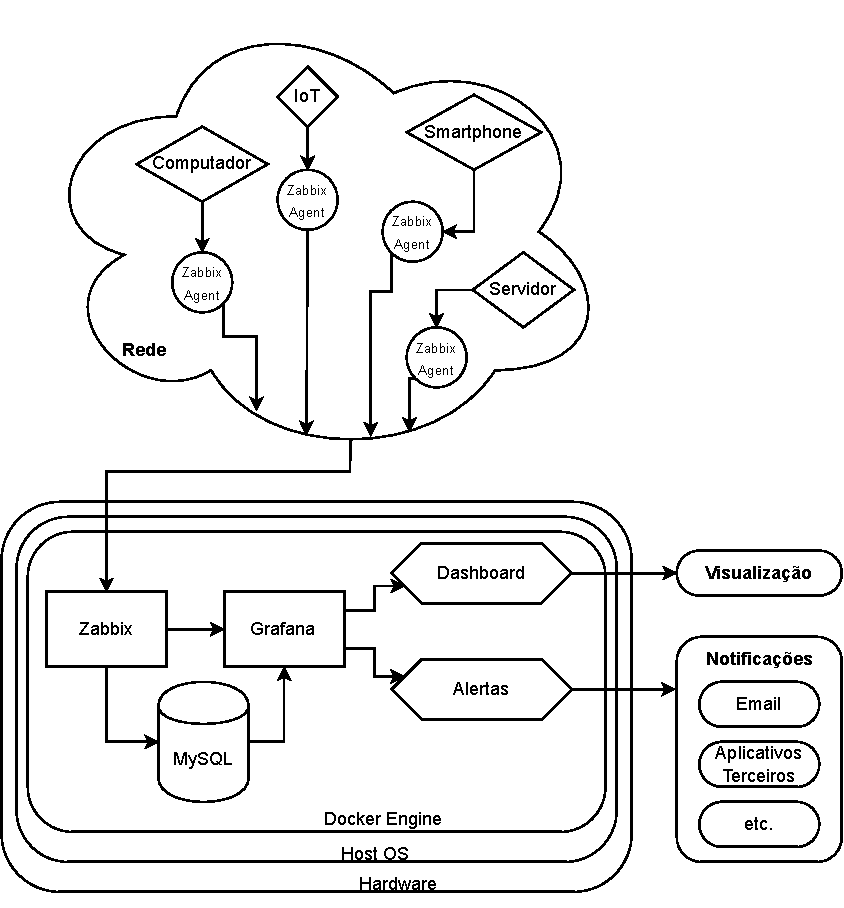
\includegraphics[scale=0.97]{Imagens/chap03/v2_diagram.pdf}
\caption{Arquitetura reformulada.}
\label{fig:ArquiteturaReformulada}
\end{figure}


\subsection{Das versões iniciais}
\label{subsection:VersõesIniciais}

A virtualização desempenha um papel essencial neste trabalho. Além dos benefícios já mencionados, a conteinerização utilizando orquestradores como Docker Compose permite o versionamento de todo o trabalho desenvolvido em repositórios de controle de versão, como o Git. Esta abordagem rege todo o trabalho a seguir.

Desde o início do projeto, o Zabbix foi escolhido como principal ferramenta de monitoramento. Mesmo após a reformulação do escopo, o Zabbix permaneceu como a solução central, devido à sua capacidade de atender todos os requisitos do projeto: possui interface web, é de código aberto, é amplamente utilizado e consolidado no mercado, sendo compatível com diversos sistemas operacionais, arquiteturas e possuindo ampla documentação e ferramentas como agentes, proxies e servidores. Além disso, o Zabbix é altamente escalável, permitindo a adição de novos dispositivos e serviços monitorados de forma simples e eficiente.

Tendo o Zabbix como sistema de monitoramento central, posteriormente aco\-plaria-se a ele o Grafana. Apesar do Zabbix já possuir uma interface web com \foreign{dashboards} e gráficos, o Grafana oferece uma experiência de visualização mais rica e personalizável, sendo um complemento ideal.

A partir do repositório Docker oficial do Zabbix  \citep{zabbixdocker2025}, fez-se um \foreign{fork} para o repositório dedicado a este projeto. Essa abordagem permitiu a experimentação com os principais recursos conteinerizados da ferramenta, como servidor Zabbix, banco de dados MySQL, e agentes. O servidor foi inicialmente configurado com um \foreign{dashboard} básico, aproveitando o modelo fornecido pelo repositório Zabbix-Docker.

Após a execução bem-sucedida dos contêineres que compunham o sistema de monitoramento central, procedeu-se à instalação de um agente Zabbix no dispositivo móvel do autor para fins de teste. Foi possível realizar o \foreign{ping} do dispositivo a partir do servidor, sendo ambos --- o agente conteinerizado e o instalado no dispositivo móvel --- devidamente adicionados à lista de \foreign{hosts} do servidor.

É importante ressaltar que o Zabbix não dispõe de agentes oficiais para dispositivos móveis, mas disponibiliza recomendações de versões não oficiais desenvolvidas por terceiros para esse tipo de aplicação.

Durante essas implementações, foram identificados alguns pontos críticos que impactaram a continuidade do Zabbix como ferramenta principal de monitoramento do projeto: a necessidade de executar um contêiner adicional exclusivamente para o banco de dados (MySQL ou Postgres) eleva o custo computacional do ambiente; a interface gráfica do Zabbix apresentou limitações quanto à navegabilidade e usabilidade, dificultando a adaptação do autor; e o projeto Zabbix-Docker, por abranger múltiplas configurações, mostrou-se extenso e complexo, o que dificultou a leitura, compreensão e manutenção do código.

Além desses aspectos, o autor enfrentava simultaneamente a curva de aprendizado do Zabbix e do Docker, o que elevou significativamente o esforço necessário para a evolução do projeto. Tal cenário levou à decisão de abandonar o Zabbix, optando-se pela adoção do Prometheus nas etapas subsequentes deste trabalho.

\begin{figure}[H]
\centering
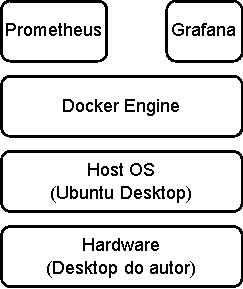
\includegraphics[scale=0.97]{Imagens/chap03/v3_stack.pdf}
\caption{\foreign{Stack} da versão-base do projeto.}
\label{fig:StackBase}
\end{figure}
\begin{figure}[H]
\centering
% \setlength{\abovecaptionskip}{-20pt}
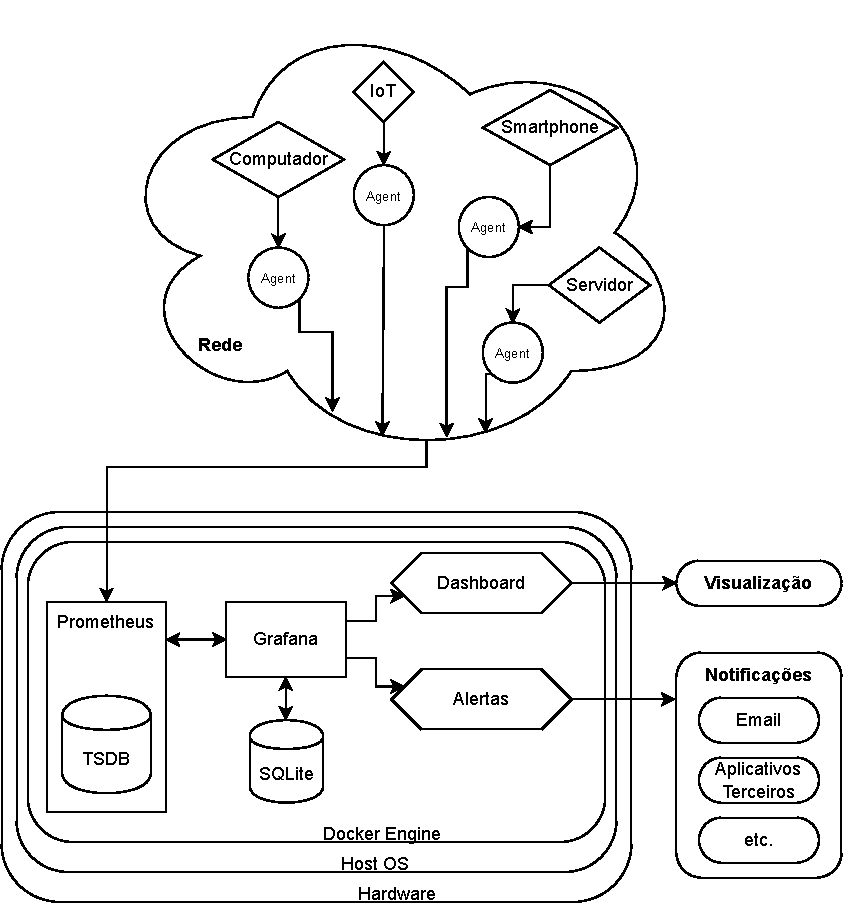
\includegraphics[scale=0.98]{Imagens/chap03/v3_diagram.pdf}
\caption{Arquitetura da versão-base do projeto.}
\label{fig:ArquiteturaBase}
\end{figure}

\section{Descrição da Arquitetura}
\label{section:DescricaoArquitetura}

Com o escopo e as ferramentas devidamente definidos, e tomando como referência a versão-base apresentada na seção anterior, esta seção descreve integralmente o trabalho desenvolvido: desde as simulações realizadas para obtenção de dados, passando pelos procedimentos de coleta e armazenamento, até a configuração dos mecanismos de visualização e alerta.

Nas subseções seguintes, são detalhados os principais blocos que compõem a arquitetura, seu funcionamento e as interações entre eles, culminando na apresentação da versão final da solução. Embora a ordem em que as subseções são apresentadas não siga estritamente a sequência cronológica do desenvolvimento, a estrutura adotada busca facilitar a compreensão do leitor, organizando o conteúdo de maneira progressiva conforme o fluxo natural de entrada, processamento e saída de dados.

\subsection{Dispositivos virtuais}
\label{subsection:DispositivosVirtuais}

\begin{figure}[H]
\centering
% \setlength{\abovecaptionskip}{-20pt}
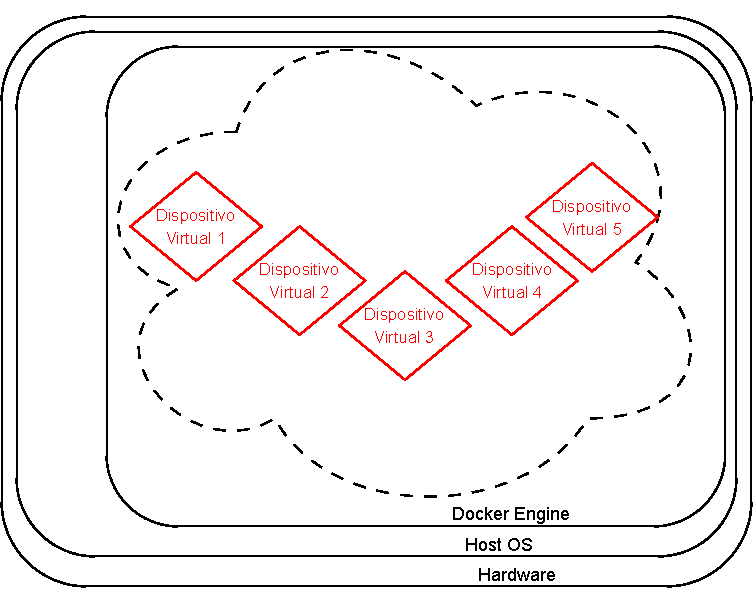
\includegraphics[scale=1]{Imagens/chap03/by-blocks/virtual_devices_diagram.pdf}
\caption{Dispositivos virtuais.}
\label{fig:DiagramaDispositivosVirtuais}
\end{figure}

Para a aquisição de dados, foram instanciados cinco contêineres Docker para simular uma rede de computadores. A fim de reproduzir um ambiente heterogêneo, cada contêiner recebeu restrições específicas de CPU e memória em sua configuração no Docker Compose. O Dockerfile, por sua vez, provisiona a distribuição Linux, \foreign{script} e software para geração de carga e o agente de monitoramento. Detalhamentos sobre essas ferramentas são apresentados nas subseções seguintes.

Além das limitações de recursos, houve também a preocupação em manter limitado o permissionamento de acesso dos contêineres à comunicação e recursos do \foreign{host}. Essa medida tem como objetivo garantir o isolamento de cada dispositivo virtual, simulando a independência típica de dispositivos reais em uma rede.

Denominados como dispositivos virtuais 1 a 5, eles foram configurados de acordo com as especificações resumidas na tabela a seguir:

\begin{table}[h]
\centering
\caption{Especificações dos dispositivos virtuais.}
\label{tab:EspecificaçõesDispositivosVirtuais}
\begin{tabular}{c c c c}
\hline
\textbf{Dispositivo Virtual} & \textbf{Distribuição Linux} & \textbf{CPU (\%)} & \textbf{Memória (MB)} \\
\hline
1 & Ubuntu 24 & 60 & 1024 \\
2 & Ubuntu 24 & 60 & 900 \\
3 & Ubuntu 24 & 70 & 800 \\
4 & Alpine 3.21 & 50 & 886 \\
5 & Alpine 3.21 & 60 & 750 \\
\hline
\end{tabular}
\end{table}

É importante destacar que o Docker, por padrão, considera 100\% de um núcleo como limite máximo de uso de CPU; logo, a atribuição de 0.6 no arquivo Compose indica que o contêiner está autorizado a utilizar até 60\% da capacidade de um único núcleo.

Os valores atribuídos às limitações de memória foram definidos a partir de cálculos estimativos, considerando a carga potencial gerada pelo \foreign{script} de geração de carga, acrescida do consumo médio do sistema operacional e do agente Telegraf. Durante os testes iniciais, esses parâmetros foram ajustados empiricamente, de modo a assegurar a operação estável dos contêineres dentro dos limites estabelecidos.

% O código fonte do Docker Compose e dos Dockerfiles empregados na criação desses dispositivos virtuais encontra-se disponível no Apêndice \ref{apendiceA}.
\break

\subsection{Agentes}
\label{subsection:Agentes}

\begin{figure}[H]
\centering
% \setlength{\abovecaptionskip}{-20pt}
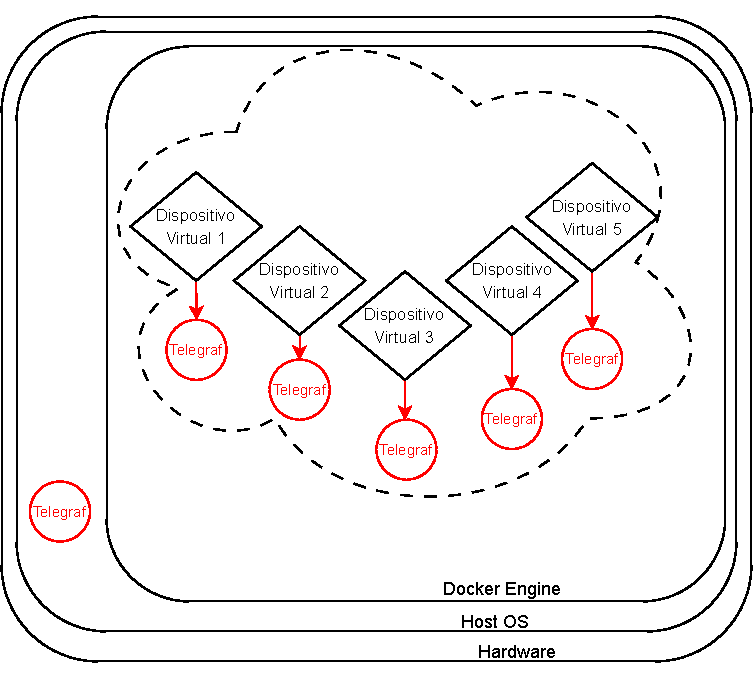
\includegraphics[scale=1]{Imagens/chap03/by-blocks/agents_diagram.pdf}
\caption{Agentes Telegraf.}
\label{fig:DiagramaAgentes}
\end{figure}

Com a substituição do Zabbix pelo Prometheus como sistema de monitoramento principal, todas as ferramentas pertencentes ao ecossistema Zabbix, inclusive seus agentes, foram descartadas. Isso tornou necessário avaliar alternativas de agentes mais adequadas ao novo contexto deste trabalho.

{\color{red}

Uma premissa importante na seleção do agente foi sua implementação dentro de cada contêiner dos dispositivos virtuais. Essa abordagem visa aproximar o ambiente de simulação de um cenário real, no qual cada dispositivo possui seu próprio agente de monitoramento. Para tanto, todos os contêineres dos dispositivos virtuais incorporam um agente por meio de sua inclusão direta no respectivo Dockerfile, garantindo consistência e uniformidade na arquitetura de monitoramento.

}
Inicialmente, conforme as recomendações da documentação do Prometheus \citep{promnodeexporter2025}, foi adotado o Node Exporter como exportador. Sua simplicidade, leveza, compatibilidade e fácil integração com o Prometheus foram destaques durante a implementação. Contudo, durante as validações iniciais, verificou-se que o Node Exporter coleta apenas métricas relacionadas ao \foreign{host}, deixando de capturar informações específicas de cada contêiner --- uma limitação incompatível com os objetivos deste trabalho.

A partir dessa constatação, foram avaliados outros agentes, como o Prometheus Agent e o Grafana Agent, mas ambos também se mostraram inadequados pelos mesmos motivos do Node Exporter. O cAdvisor, outro agente de monitoramento bastante utilizado, chegou a ser considerado, porém sua abordagem operacional não está alinhada à premissa do projeto, pois opera num contêiner próprio e coleta métricas diretamente do Docker \foreign{daemon}, sem a necessidade de instalação individual em cada contêiner. Apesar de sua eficiência, essa solução não atende aos requisitos deste trabalho, que exige uma arquitetura consistente tanto para dispositivos virtuais quanto reais. Os motivos que levaram à desistência do cAdvisor também fundamentaram a rejeição ao Docker Stats Exporter, um exportador que chegou a ser avaliado durante o desenvolvimento.

Outra premissa importante na busca por minimização de distorções e vieses nas leituras é a utilização de um agente versátil, capaz de operar em diversos tipos de sistemas e dispositivos. A partir das premissas apresentadas e das limitações encontradas nos agentes já mencionados, o Telegraf emergiu como a solução ideal para atender às necessidades impostas.

Altamente configurável, o Telegraf pode ser facilmente integrado a diferentes sistemas e dispositivos, além de possuir suporte nativo para o Prometheus. Sua flexibilidade permite a coleta de uma ampla gama de métricas, tanto do \foreign{host} quanto dos contêineres. Além disso, suas popularidade, documentação e compatibilidade com diversas plataformas facilitam sua adoção e manutenção. Cabe ressaltar que o Telegraf apresenta um custo computacional superior ao do Node Exporter. Esse impacto pode ser ainda maior dependendo dos \foreign{plugins} utilizados.

Instalou-se uma instância do Telegraf em cada contêiner de dispositivo virtual (via Dockerfile) e, adicionalmente, uma instância no \foreign{host} do projeto, com a finalidade de enriquecer os dados coletados. Para garantir uma configuração padronizada, foram definidos dois arquivos \verb|telegraf.conf| distintos: um aplicado aos contêineres e outro ao \foreign{host}.

As configurações foram escritas em formato TOML \abbrev{TOML}{\foreign{Tom's Obvious, Minimal Language}}, de modo que todos os dispositivos compartilham os mesmos parâmetros globais e de saída. Já as configurações de entrada foram ajustadas conforme o papel de cada instância -- diferenciando o \foreign{host} dos dispositivos virtuais.

Descrições mais detalhadas podem ser encontradas nos apêndices \textcolor{blue}{incluir apêndices}. Destaca-se, entretanto, os parâmetros: o uso de \verb|interval = "5s"|, que define a coleta de métricas a cada cinco segundos -- em sincronia com o intervalo de \foreign{scraping} do Prometheus -- e a utilização do \foreign{plugin} \verb|outputs.prometheus_client|, que expõe as métricas no formato Prometheus, permitindo ao mesmo realizar o \foreign{scraping} no \foreign{endpoint} \verb|/metrics| do Telegraf.

Quanto às configurações de entrada, o arquivo \verb|telegraf.conf| do \foreign{host} emprega \foreign{plugins} específicos para cada categoria de métricas: \verb|inputs.cpu|, \verb|inputs.mem|, \verb|inputs.disk|, \verb|inputs.diskio|, \verb|inputs.net| e \verb|inputs.processes|. Essa estratégia otimiza a coleta de dados, ao empregar \foreign{plugins} específicos para cada recurso, além de simplificar a manutenção e favorecer a escalabilidade da solução

Para os dispositivos virtuais, foi inicialmente empregado o \foreign{plugin} \verb|inputs.exec|, que cria \foreign{threads} periodicamente para executar comandos específicos e coletar as métricas desejadas. As especificações de tipagem dos dados, os comandos a serem executados e a formatação das saídas eram definidas manualmente no arquivo \verb|telegraf.conf|. Embora essa abordagem seja funcional, revelou-se pouco eficiente devido à sua complexidade, ao elevado custo computacional --- decorrente da constante criação de novas \foreign{threads} --- e à dificuldade de manutenção, pois qualquer alteração exigia modificações manuais no arquivo de configuração.

No contexto da coleta de métricas, os \foreign{plugins} mencionados realizam a leitura de arquivos exclusivamente relacionados ao \foreign{kernel} do \foreign{host} (com exceção do \verb|inputs.net| e \verb|inputs.processes|), o que os torna inadequados para uso em contêineres, dadas as restrições de permissões de acesso ao \foreign{host}. Em busca de alternativas, o \foreign{plugin} \verb|inputs.docker| foi considerado, pois permite a coleta de métricas diretamente do \foreign{socket} do Docker \foreign{daemon}. No entanto, essa solução não é compatível com o Telegraf executando dentro de um contêiner, uma vez que o acesso ao \foreign{socket} do Docker exige permissões elevadas junto ao \foreign{host}, contrariando as premissas de isolamento estabelecidas para os dispositivos virtuais.

Por fim, considerando as limitações discutidas, optou-se pelo uso do \foreign{plugin} \verb|inputs.cgroups|, que é especializado na leitura dos arquivos presentes no \foreign{path} \verb|/sys/fs/cgroups| do Linux --- os mesmos utilizados pelo Docker para gerenciar e monitorar contêineres. Essa solução permite a coleta precisa de métricas diretamente relacionadas aos contêineres, assegurando a qualidade dos dados sem exigir permissões elevadas de acesso ao \foreign{host}. Além disso, o \verb|inputs.cgroups| simplifica significativamente a configuração e manutenção do Telegraf, eliminando a necessidade de ajustes manuais extensivos, e reduz o custo computacional, já que não há criação recorrente de novas \foreign{threads}.

% \newpage

\begin{lstlisting}[caption={Leitura do arquivo "cpu.pressure" com inputs.exec}, label={lst:trecho1}]
[[inputs.exec]]
  commands = ["cat /sys/fs/cgroup/cpu.pressure"]
  data_format = "grok"
  grok_patterns = ["%{WORD:pressure_type} avg10=%{NUMBER:avg10:float} avg60=%{NUMBER:avg60:float} avg300=%{NUMBER:avg300:float} total=%{NUMBER:total:int}"]
  timeout = "5s"
\end{lstlisting}

\begin{lstlisting}[caption={Leitura do mesmo arquivo "cpu.pressure" com inputs.cgroups}, label={lst:trecho2}]
[[inputs.cgroup]]
  paths = ["/sys/fs/cgroup/"]
  files = [
    "cpu.pressure"
  ]
\end{lstlisting}


% Diretivas globais:

% \begin{table}[h!]
% \centering
% \begin{tabular}{|l|p{10cm}|}
% \hline
% \textbf{Configuração} & \textbf{Descrição (PT-BR)} \\
% \hline
% \textbf{interval = "5s"} & Coleta métricas a cada 5 segundos (alinhado com Prometheus). \\
% \hline
% \textbf{round\_interval = true} & Alinha a coleta com múltiplos exatos do intervalo. \\
% \hline
% \textbf{metric\_batch\_size = 1000} & Envia até 1000 métricas por lote para os outputs. \\
% \hline
% \textbf{metric\_buffer\_limit = 10000} & Armazena até 10000 métricas em buffer caso haja falha de scraping. \\
% \hline
% \textbf{collection\_jitter = "0s"} & Sem atraso aleatório na coleta (maior precisão temporal). \\
% \hline
% \textbf{flush\_interval = "5s"} & Descarrega métricas a cada 5 segundos (mesmo ritmo da coleta). \\
% \hline
% \textbf{flush\_jitter = "0s"} & Sem atraso aleatório no envio (saída determinística). \\
% \hline
% \textbf{precision = "0s"} & Mantém precisão total do timestamp (nanosegundos). \\
% \hline
% \textbf{debug = false} & Desabilita logs de depuração (reduz verbosidade em produção). \\
% \hline
% \textbf{quiet = false} & Mantém logging padrão (não fica silencioso). \\
% \hline
% \textbf{logfile = ""} & Usa syslog/systemd para logs (sem arquivo dedicado). \\
% \hline
% \textbf{hostname = ""} & Usa o hostname real do sistema. \\
% \hline
% \textbf{omit\_hostname = false} & Inclui a tag \texttt{host} nas métricas. \\
% \hline
% \textbf{listen = ":9273"} & Servidor HTTP interno escuta na porta 9273 para Prometheus. \\
% \hline
% \textbf{path = "/metrics"} & Endpoint HTTP onde métricas são expostas. \\
% \hline
% \textbf{expiration\_interval = "120s"} & Remove métricas que não se atualizam por 120s. \\
% \hline
% \textbf{metric\_version = 2} & Usa formato v2 de métricas Prometheus (nomenclatura melhorada). \\
% \hline
% \end{tabular}
% \end{table}

% \begin{itemize}
%   \item \textbf{interval = "5s"}: Coleta métricas a cada 5 segundos (alinhado com Prometheus).
%   \item \textbf{round\_interval = true}: Alinha a coleta com múltiplos exatos do intervalo.
%   \item \textbf{metric\_batch\_size = 1000}: Envia até 1000 métricas por lote para os outputs.
%   \item \textbf{metric\_buffer\_limit = 10000}: Armazena até 10000 métricas em buffer caso haja falha de scraping.
%   \item \textbf{collection\_jitter = "0s"}: Sem atraso aleatório na coleta (maior precisão temporal).
%   \item \textbf{flush\_interval = "5s"}: Descarrega métricas a cada 5 segundos (mesmo ritmo da coleta).
%   \item \textbf{flush\_jitter = "0s"}: Sem atraso aleatório no envio (saída determinística).
%   \item \textbf{precision = "0s"}: Mantém precisão total do timestamp (nanosegundos).
%   \item \textbf{debug = false}: Desabilita logs de depuração (reduz verbosidade em produção).
%   \item \textbf{quiet = false}: Mantém logging padrão (não fica silencioso).
%   \item \textbf{logfile = ""}: Usa syslog/systemd para logs (sem arquivo dedicado).
%   \item \textbf{hostname = ""}: Usa o hostname real do sistema.
%   \item \textbf{omit\_hostname = false}: Inclui a tag \texttt{host} nas métricas.
%   \item \textbf{listen = ":9273"}: Servidor HTTP interno escuta na porta 9273 para Prometheus.
%   \item \textbf{path = "/metrics"}: Endpoint HTTP onde métricas são expostas.
%   \item \textbf{expiration\_interval = "120s"}: Remove métricas que não se atualizam por 120s.
%   \item \textbf{metric\_version = 2}: Usa formato v2 de métricas Prometheus (nomenclatura melhorada).
% \end{itemize}

\subsection{Prometheus e TSDB}
\label{subsection:PrometheusTSDB}

\begin{figure}[H]
\centering
% \setlength{\abovecaptionskip}{-20pt}
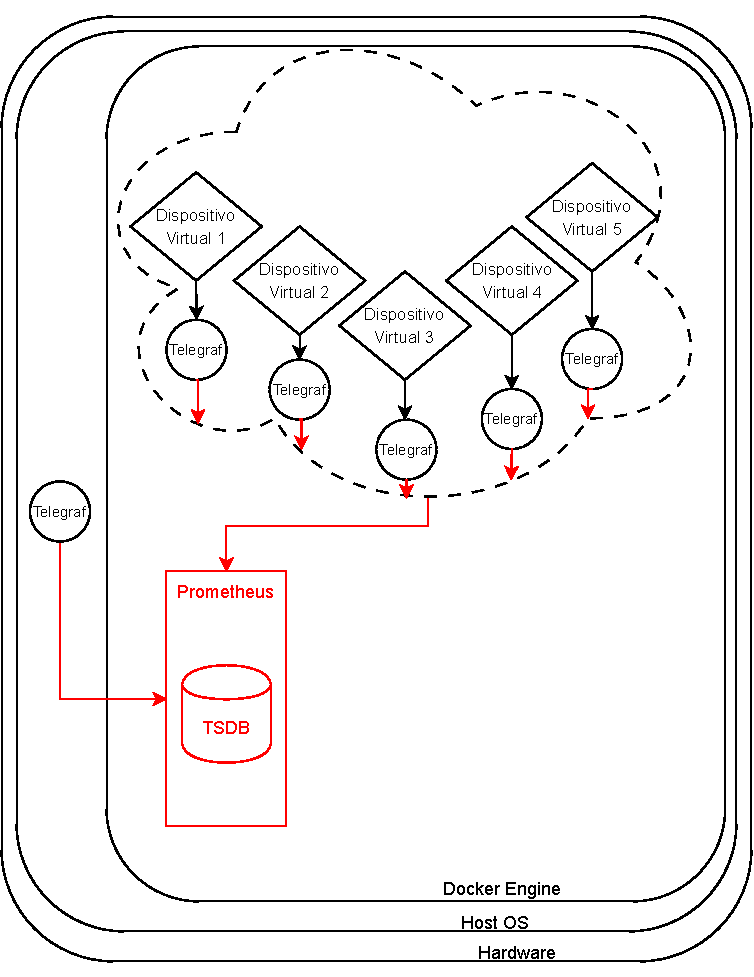
\includegraphics[scale=1]{Imagens/chap03/by-blocks/prometheus_diagram.pdf}
\caption{Prometheus e TSDB.}
\label{fig:DiagramaPrometheusTSDB}
\end{figure}

Para implementar o sistema de monitoramento central, o serviço Prometheus foi adicionado ao Docker Compose. Essa inclusão trouxe não apenas o ferramental para coleta das métricas expostas pelos agentes Telegraf, mas também o banco de dados de séries temporais (TSDB), responsável pelo armazenamento permanente dessas métricas. Como o TSDB é parte integrante do Prometheus, não foi necessária nenhuma configuração adicional para sua integração, o que não só simplificou significativamente a implementação como também reduziu o custo e otimizou o desempenho do sistema.

No Compose, além das diretivas comuns de configuração de contêineres --- como mapeamento de portas, redes e volumes --- destacam-se as diretivas \verb|extra_hosts| e \verb|command|. A primeira permite que o contêiner do Prometheus consiga acessar o host da máquina onde está sendo executado, configuração fundamental para coleta das métricas do agente Telegraf em execução no host. A segunda, por sua vez, configura o tempo de retenção dos dados no TSDB para 15 dias, utilizando o comando \verb|--storage.tsdb.retention.time=15d|.

Já no arquivo \verb|prometheus.yml|, são definidas as regras globais de \textcolor{red}{\foreign{scraping}} \textcolor{blue}{O termo \foreign{scraping} é apresentado e traduzido lá no capítulo 2 em \ref{subsection:Prometheus}. É inclusive utilizado nas documentações oficiais. Eu acho que "extração de dados" passa uma noçao de que o prometheus vai lá na fonte ativamente pegar os dados, quando na verdade o que ele faz é a \foreign{raspagem} dos endpoints do telegraf. Podemos discutir melhor na terça}, os direcionamentos para o arquivo de regras e para o serviço de alertas (Alertmanager -- a ser detalhado posteriormente), além das configurações dos \foreign{endpoints} do Telegraf para coleta de dados. Ressalta-se que, em \verb|global|, o parâmetro \verb|scrape_interval| é definido como 5 segundos, enquanto o \verb|scrape_timeout| é ajustado para 4 segundos. Essa configuração proporciona uma coleta de alta frequência, permitindo maior granularidade dos dados. Ao mesmo tempo, o limite de 4 segundos para o tempo de requisição evita bloqueios prolongados: caso uma coleta exceda esse tempo, o Prometheus considera a tentativa como falha e parte para uma nova coleta no próximo intervalo, o que contribui para a prevenção de congestionamentos no sistema.

Além disso, há uma importante sincronia entre os intervalos de \foreign{scraping} do Prometheus e os de coleta do Telegraf --- ambos configurados para 5 segundos. Essa equivalência garante que as métricas coletadas estejam sempre atualizadas e alinhadas entre as duas ferramentas.

\subsection{Grafana}
\label{subsection:GrafanaVisualizacao}

\begin{figure}[H]
\centering
% \setlength{\abovecaptionskip}{-20pt}
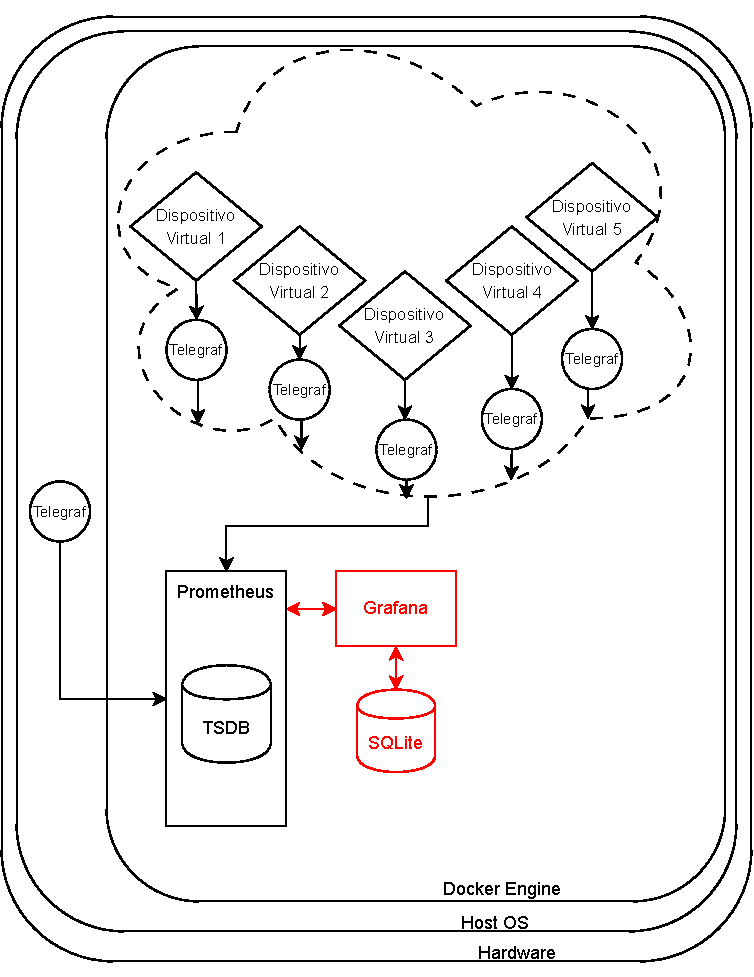
\includegraphics[scale=1]{Imagens/chap03/by-blocks/grafana_diagram.pdf}
\caption{Grafana}
\label{fig:DiagramaGrafana}
\end{figure}

Como mencionado no Capítulo \ref{chap2}, o Prometheus Expression Browser oferece uma interface web básica para visualização de métricas, porém essa interface apresenta limitações e não atende às demandas para visualizações avançadas. Por esse motivo, o próximo passo do projeto foi integrar o Grafana.

Assim como nos demais serviços, a inclusão do Grafana ao Docker Compose envolveu apenas a definição das configurações básicas. Neste caso, é importante destacar a utilização da diretiva \verb|volumes|, que aponta para dois caminhos específicos: \verb|grafana/dashboard-json| e \verb|grafana/provisioning|. O primeiro armazena os arquivos JSON dos \foreign{dashboards}, que serão importados automaticamente pelo Grafana durante a inicialização. O segundo contém as configurações de provisionamento, usadas para automatizar a integração de fontes de dados e \foreign{dashboards}. Esse mecanismo é essencial para a automação do projeto, pois garante que todas as configurações necessárias --- tanto das integrações com fontes de dados, como o Prometheus, quanto dos \foreign{dashboards} --- sejam carregadas automaticamente ao iniciar o contêiner, dispensando procedimentos manuais pela interface web.

Adicionalmente, a imagem oficial do Grafana utilizada no projeto já inclui o banco de dados SQLite, responsável por armazenar as configurações realizadas por meio da interface gráfica. As configurações aplicadas via provisionamento são acessíveis em modo \foreign{read-only} na interface e não podem ser modificadas manualmente. Já as alterações feitas diretamente pela interface gráfica são gravadas no SQLite, mas não são replicadas para os arquivos de provisionamento nem registradas em versionamento. Em situações de conflito entre as configurações do provisionamento e as definidas pela interface gráfica, prevalecem aquelas estabelecidas pelo provisionamento.

\subsection{Testes de saturação}
\label{subsection:TestesSaturacao}

\begin{figure}[H]
\centering
% \setlength{\abovecaptionskip}{-20pt}
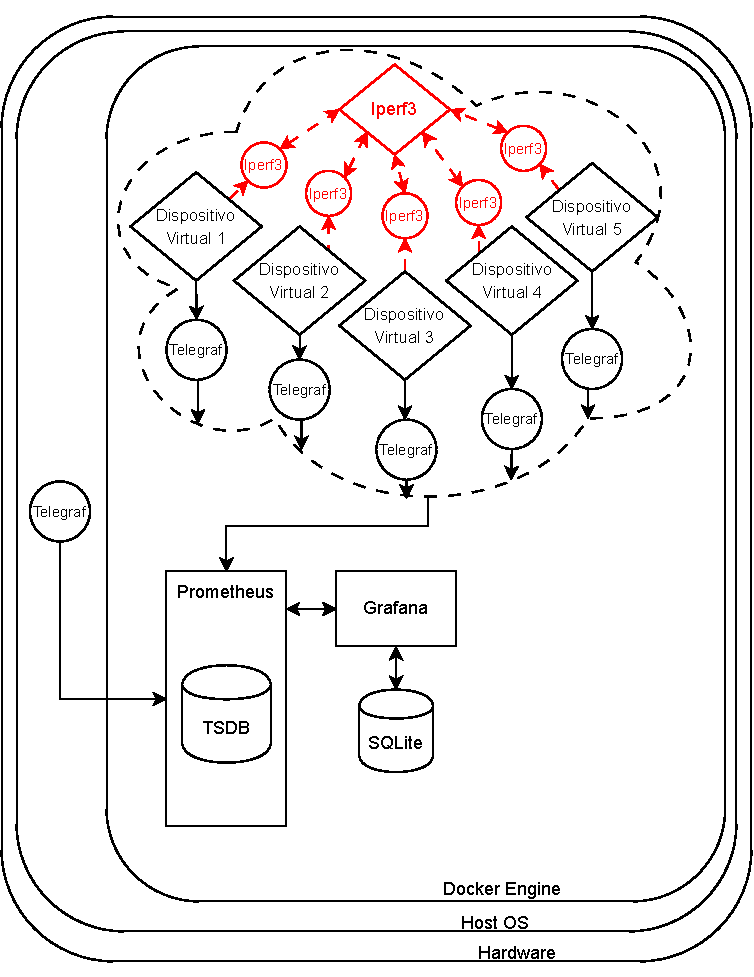
\includegraphics[scale=1]{Imagens/chap03/by-blocks/saturation_diagram.pdf}
\caption{Ferramentas de saturação.}
\label{fig:DiagramaSaturacao}
\end{figure}

Os dispositivos virtuais, por si só, não produzem dados suficientes para uma análise qualitativa ou quantitativa eficaz do sistema de monitoramento. Por esse motivo, foram implementados testes de saturação, consistindo na geração de carga adicional sobre os dispositivos virtuais para simular cenários de uso intenso e coletar as métricas correspondentes.

Inicialmente, a introdução de carga foi realizada exclusivamente com o stress-ng, integrado aos Dockerfiles dos dispositivos virtuais. Posteriormente, desenvolveu-se um \foreign{script} Bash que executa o stress-ng com diferentes parâmetros, simulando variados tipos de carga (CPU, memória, I/O, etc.) e níveis de intensidade. Esse \foreign{script} é executado em segundo plano, simultaneamente à execução do agente Telegraf, garantindo a geração contínua de carga durante a coleta das métricas.

Apesar do bom desempenho na geração de carga computacional, o stress-ng mostrou-se insuficiente para simular tráfego de rede de forma realista. Para superar essa limitação, foi incorporado o iPerf3 ao projeto. Como esta ferramenta opera no modelo cliente-servidor e não permite a atuação simultânea nessas funções, foi criado um contêiner dedicado para funcionar como servidor iPerf3. Em paralelo, cada dispositivo virtual passou a contar com uma instância do iPerf3 configurada como cliente. Dessa maneira, tornou-se possível gerar tráfego de rede entre os dispositivos virtuais e o servidor iPerf3, aprimorando a simulação de carga sobre o ambiente de rede.


\begin{figure}[H]
\centering
% \setlength{\abovecaptionskip}{-10pt}
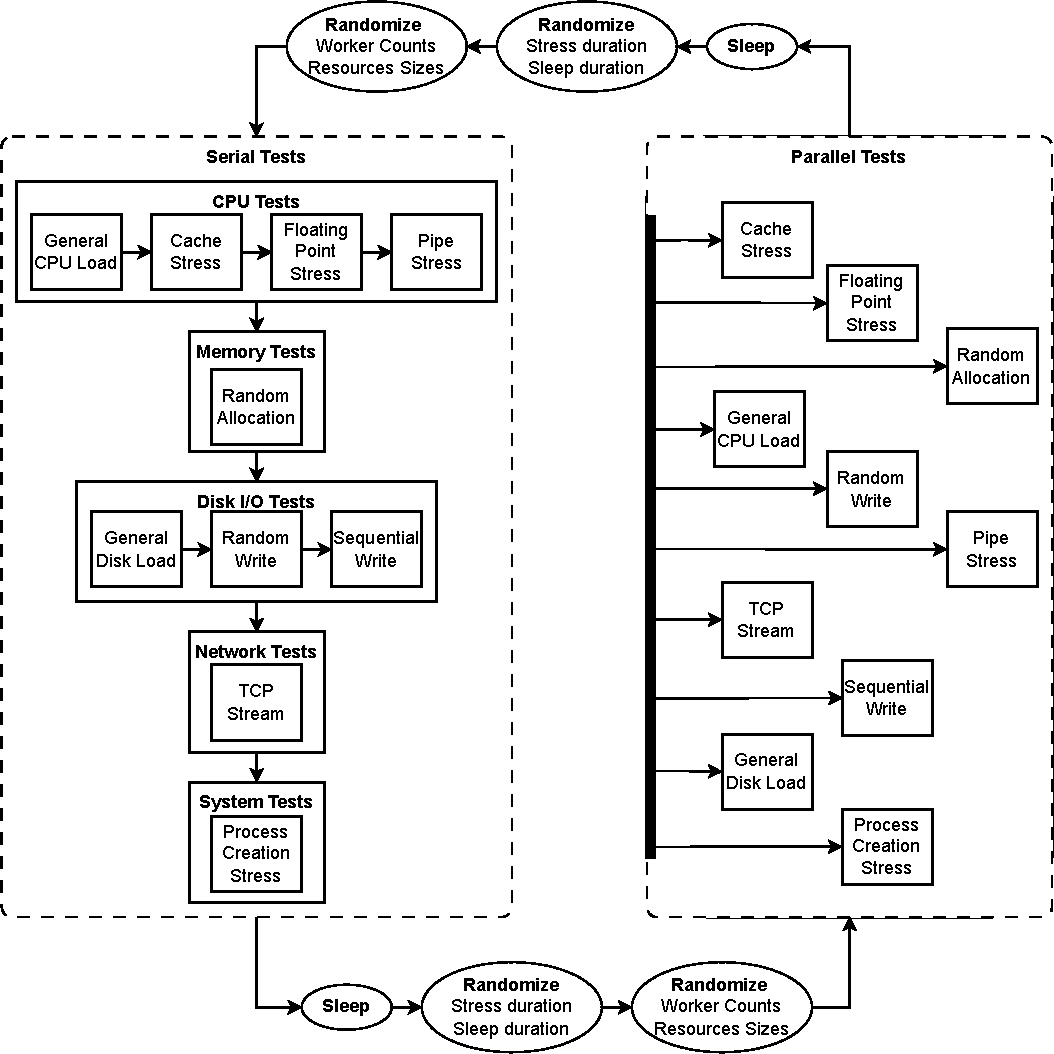
\includegraphics[scale=0.75]{Imagens/chap03/load_generator_flowchart2.pdf}
\caption{Fluxograma dos testes de carga.}
\label{fig:FluxogramaCarga}
\end{figure}



O script executa um \foreign{loop} \verb|while true| estruturado em dois blocos principais: inicialmente, realiza uma série de testes sequenciais, seguidos pela repetição desses testes de forma paralela e simultânea. No início de cada bloco, os valores de duração dos testes (\verb|stress_time|) e do tempo de espera entre um bloco e outro (\verb|sleep_time|) são definidos aleatoriamente. {\color{red}Ao término dos testes paralelos, aguarda-se o \verb|sleep_time| previamente estabelecido e, em seguida, inicia-se um novo ciclo, conforme ilustrado no fluxograma da Figura \ref{fig:FluxogramaCarga}. Esse processo se repete indefinidamente, possibilitando a execução contínua dos testes de saturação até que ocorra uma intervenção manual ou a finalização do contêiner.}

A aleatoriedade nas durações dos testes e dos intervalos de espera, bem como a definição contínua de novos valores a cada execução de bloco, tem como objetivo conferir um caráter caótico aos experimentos, aproximando-os das condições reais de operação. Embora os valores sejam determinados aleatoriamente, eles obedecem a intervalos previamente estabelecidos: nos testes sequenciais, cada execução ocorre entre 15 e 20 segundos; no bloco paralelo, o tempo total de execução varia de 25 a 30 segundos. Para ambos os blocos, o intervalo de espera entre execuções está fixado entre 10 e 30 segundos.

Além da aleatoriedade nas durações, a carga aplicada nos testes também é definida de maneira aleatória. No stress-ng, essa carga corresponde ao número de \foreign{workers}, ou seja, processos ou \foreign{threads} inicializados para executar os testes. Antes de cada execução de bloco, novas cargas são estabelecidas. Nas figuras os \foreign{scripts} são representados pelo símbolo 
\includegraphics[height=1em]{Imagens/chap03/input_black.png}. 

\subsection{Desafios na Integração de Dispositivos Móveis}
\label{subsection:DesafiosDispositivosMoveis}

Diversas tentativas de incluir dispositivos móveis na rede de monitoramento foram realizadas ao longo do desenvolvimento, com o intuito de ampliar a diversidade dos equipamentos monitorados. No entanto, obstáculos técnicos --- como a ausência de suporte oficial para Android e restrições de permissão do sistema operacional (incluindo limitações de segurança e necessidade de acesso \foreign{root}) --- inviabilizaram essa integração. Embora não tenham se mostrado viáveis, essas experiências contribuíram para um melhor entendimento das limitações e desafios envolvidos no monitoramento de dispositivos móveis.

Destaca-se que, em uma das tentativas, foi possível realizar com êxito um \foreign{ping} ao dispositivo móvel do autor, equipado com uma versão não oficial do Zabbix Agent recomendada pela própria Zabbix \citep{unofficialzabbixagent2025}, via contêiner do servidor Zabbix (anterior à adoção do Prometheus). Ainda assim, as dificuldades anteriormente expostas impediram o avanço dessa abordagem.

Considerou-se também a utilização do \foreign{agentless monitoring} (monitoramento sem agentes) por meio do SNMP, mas essa alternativa foi descartada devido à complexidade adicional e às limitações do protocolo, como a necessidade de pré-configuração nos dispositivos e a restrição quanto ao tipo e à quantidade de métricas acessíveis.

Também estudou-se a simulação de dispositivos móveis por meio de emuladores Android, alternativa igualmente abandonada devido ao aumento da complexidade do projeto.


\section{Infraestrutura}
\label{section:Infraestrutura}

Ao longo do projeto, dois equipamentos estiveram à disponibilidade do autor: um desktop pessoal e um \foreign{notebook} corporativo, conforme mencionado em \ref{subsection:EscopoReformulado}. As especificações desses equipamentos estão detalhadas na Tabela \ref{tab:available-hardware}.

\begin{table}[H]
\centering
\caption{Especificações de hardware dos equipamentos disponíveis}
\label{tab:available-hardware}
\begin{tabular}{lcc}
\toprule
\textbf{Componente} & \textbf{Desktop} & \textbf{Notebook} \\
\midrule
CPU   & Intel Core i5-7600   & Intel Core i7-8565U \\
RAM   & 16GB                 & 32GB                \\
Disco & 500GB (SSD)            & 250GB (SSD)          \\
SO & Ubuntu Desktop 24 & Ubuntu Desktop 20 \\
\bottomrule
\end{tabular}
\end{table}

As práticas adotadas ao longo deste projeto possibilitaram um desenvolvimento multi-máquina prático e eficiente. Cada equipamento implementou o projeto por meio de clones locais do repositório e executou os mesmos comandos Docker Compose para iniciar toda a infraestrutura de monitoramento. A possibilidade de rodar o mesmo projeto em diferentes máquinas, sem necessidade de instalações manuais ou configurações complexas, destacou-se como uma das principais vantagens do desenvolvimento.

A escolha do Ubuntu Desktop como sistema operacional base para ambos os equipamentos foi motivada por sua estabilidade, ampla adoção na comunidade de desenvolvedores e compatibilidade com as ferramentas utilizadas no projeto, onde o \foreign{notebook} operava com a versão 20 e o \foreign{desktop} com a versão 24.

Entretanto, a partir de determinado momento, o \foreign{desktop} começou a apresentar instabilidades e travamentos de origem desconhecida. Esses problemas tiveram impacto negativo na coleta de dados e, consequentemente, nas visualizações, ocasionando \foreign{gaps} nas curvas dos gráficos e perda de informações. Diante desse contexto, decidiu-se consolidar o \foreign{notebook} como equipamento principal para o desenvolvimento do projeto, descartando o uso do \foreign{desktop}.



\section{Discussão sobre as métricas}
\label{section:DiscussaoMetricas}
{\color{red}
As métricas apresentadas neste trabalho são extraídas por meio da leitura de arquivos de sistema do Linux. Particularmente para métricas de CPU, memória e disco dos dispositivos virtuais, a coleta ocorre a partir de arquivos localizados no diretório \verb|/sys/fs/cgroup|.

Durante o desenvolvimento multi-máquina, especialmente na etapa de configuração manual dos parâmetros do \verb|inputs.exec| do Telegraf, foram identificadas inconsistências e erros na leitura das métricas entre as implementações feitas no \foreign{notebook} e no \foreign{desktop}. Como apresentado em \ref{section:Infraestrutura}, o fato do \foreign{notebook} operar com o Ubuntu 20 implica que, por padrão, o mesmo apresenta a versão 1 do \foreign{cgroups}, enquanto o \foreign{desktop}, com Ubuntu 24, utiliza a versão 2.

A disparidade entre versões do \foreign{cgroups} resultou em diferenças estruturais nos arquivos de leitura das métricas, impossibilitando o uso de um arquivo de configuração único e padronizado devido a falhas recorrentes na coleta. Esse problema foi solucionado com a atualização do \foreign{cgroups} do \foreign{notebook} para a versão 2, harmonizando as estruturas dos arquivos e, consequentemente, permitindo a padronização das configurações de coleta. Cabe ressaltar que a versão do \foreign{cgroups} dos dispositivos virtuais é determinada pelo \foreign{kernel} do \foreign{host}, razão pela qual todos também passaram a operar na versão 2 após a atualização.


A seleção das métricas a serem monitoradas pautou-se nos seguintes critérios:
\begin{enumerate}
\item \textbf{Multiplataforma}: Foram priorizadas métricas disponíveis em diferentes sistemas operacionais, sendo desconsideradas aquelas exclusivas de uma plataforma específica, como as restritas ao Linux.
\item \textbf{Relevância}: As métricas escolhidas devem fornecer informações essenciais para o monitoramento da saturação do sistema, permitindo tanto a detecção imediata de problemas e a adoção de medidas corretivas quanto o auxílio a análises mais aprofundadas.
\item \textbf{Comparabilidade}: Sempre que possível, optou-se por métricas comparáveis entre os dispositivos virtualizados e físicos. Embora nem todas apresentem correspondência exata, buscou-se garantir um nível de equivalência. Ressalta-se, contudo, que algumas métricas importantes --- como determinadas métricas de disco --- não estão disponíveis nos dispositivos virtuais, mas foram mantidas pela sua relevância para o monitoramento.
\end{enumerate}

A partir dos critérios estabelecidos, e as respectivas descrições apresentadas na Seção \ref{section:Metricas} do Capítulo 2, são obtidas as seguintes métricas, a partir da leitura direta dos arquivos de sistema:

\textcolor{blue}{Estou com dificuldades de montar esta tabela \ref{tab:metricas-selecionadas} de uma forma intuitiva}
\begin{table}[H]
\color{blue}
\centering
\caption{Métricas selecionadas de leitura direta.}
\label{tab:metricas-selecionadas}
\begin{tabular}{|c|c|c|c|}
\hline
\textbf{Categoria} & \textbf{Métrica} & \textbf{Host} & \textbf{Dispositivo Virtual} \\ \hline
\multirow{4}{*}{CPU} & user & usage\_user & user\_usec \\ \cline{2-4}
                     & system & usage\_system & system\_usec \\ \cline{2-4}
                     & iowait & usage\_iowait & -- \\ \cline{2-4}
                     & idle & usage\_idle & -- \\ \hline
\multirow{4}{*}{Memória} & used & used        & memory.current                      \\ \cline{2-4}
                         & total & total       & memory.max                          \\ \cline{2-4}
                         & swap\_free & swap\_free  & memory.swap.max - memory.swap.current                     \\ \cline{2-4}
                         & swap\_total & swap\_total & memory.swap.max \\ \hline
\multirow{7}{*}{Disco} & Espaço Livre & free         & --     \\ \cline{2-4}
                       & Espaço Utilizado & used         & --     \\ \cline{2-4}
                       & Espaço Total & total        & --     \\ \cline{2-4}
                       & INODES Livres & inodes\_free & --     \\ \cline{2-4}
                       & Bytes Lidos & read\_bytes  & rbytes \\ \cline{2-4}
                       & Bytes Escritos & write\_bytes & wbytes \\ \cline{2-4}
                       & Utilização I/O & io\_util     & --     \\ \hline
\multirow{8}{*}{Rede} & Placeholder & bytes\_recv     & Bytes Received   \\ \cline{2-4}
                      & Placeholder & bytes\_sent     & Bytes Sent       \\ \cline{2-4}
                      & Placeholder & packets\_recv   & Packets Received \\ \cline{2-4}
                      & Placeholder & packets\_sent   & Packets Sent     \\ \cline{2-4}
                      & Placeholder & drop\_in        & Drop In          \\ \cline{2-4}
                      & Placeholder & drop\_out       & Drop Out         \\ \cline{2-4}
                      & Placeholder & err\_in         & Error In         \\ \cline{2-4}
                      & Placeholder & err\_out        & Error Out        \\ \hline
\multirow{4}{*}{Processos} & Em execução & running  & running  \\ \cline{2-4}
                           & Em espera & sleeping & sleeping \\ \cline{2-4}
                           & Total & total    & total    \\ \cline{2-4}
                           & Zumbi & zombies  & zombies  \\ \hline
\end{tabular}
\end{table}

\textcolor{blue}{Eu estou sentindo falta de algo para fechar esta seção, mas não sei bem o que é. Alguma sugestão? Ou acha que está suficiente?}

}



\section{Aplicação de Monitoramento}

{\color{blue}
Seção dividida em 2 partes principais:

1 - o dashboard e seus painéis

2 - alertas e notificações

3 - Acho que vai ficar muito grande, talvez pudesse virar um novo capítulo?

\textbf{Dashboards}
\begin{enumerate}  
  \item comentar sobre sobre as coisas que o provisioning já adiantou (datasource padrão, por exemplo);
  \item a normalização dos dados usando o Pormetheus Recording Rules
  \item Criação dos filtros globais;
  \item Regras globais (span e refresh rate);
  \item Falar de cada gráfico, justificando visualizações, comentando sobre as queries/cálculos e colocar imagens;
  \item Quando chegar na seção de disco, apresentar o estudo de caĺculo do df (motivação e resultados);
  \item Chegando na parte de redes, justificar o porquê de nao termos dados de drop e erro de pacotes (apresentar o estudo de caso de camadas de rede e aplicação);
  \item Fechamento explicando a exportação do JSON e seu versionamento e carregamento automatico via docker volume;
\end{enumerate}
\textbf{Alarmes e Notificações}
\begin{enumerate}
  \item Comentar sobre o Alertmanager e a sua configuração;
  \item Explicar como adicionei o servidor smtp do gmail e as tentativas falhas com o Telegram;
  \item Configuração das regras de notificação e os pontos de contato;
  \item Como utilizei, a primeiro momenot, a UI do Grafana para criar os alertas (isso era interessante pq vinculava automaticamente o alerta ao respectivo gráfico);
  \item Como, assim como no dashboard, eu exportava e versionava tudo via JSON;
  \item Problemas do SQLite e a migração para o Postgres (explicitar como a migração foi fácil graças ao provisionamento, versionamento, uso do Docker e TSDB fazendo o trabalho de persistência);
  \item Eventual abandono do Postgres e rollback para SQLite, e a migração para o Alertmanager+TSDB (enfatizar como tudo fica embutido no Prometheus e como isso simplifica a arquitetura);
\end{enumerate}


}
% \textcolor{blue}{Dúvida: Como combinamos de contar a experiencia com o SQLitexPostgres e tambem a alteração para Alertmanager na seção 3.5 (alertas e dashboards), confesso que não sei mais o que colocar aqui... talvez matemos essa subseção 3.2.6?}

% Uma dúvida que tive hoje nesta seção: nós combinamos de comentar sobre dashboards e alertas na seção 3.5, porém isso implica que eu não incluiria os respectivos blocos de dashboards e alertas (e Alertmanager) no diagrama neste momento. Isso implica que a figura do diagrama final da arquitetura só apareceria no fim da seção 3.6. Como proceder?

% Aqui a finalizo a seção contando a historia do SQLite x Postgres e eventualmente chegando na decisão de descartar ambos e ficar apenas com o TSDB.
% Tambem relato da minha experiencia de formatar a maquina toda e a facilidade em subir todo o projeto (salve a configuração pontual do permissionamento de escrita do grafana e da chave do repositorio do telegraf)
% Após isso eu fecho a seção com o diagrama da arquitetura final definitiva. 


% foram feitas tentativas de utilização de ferramentas de \foreign{chaos-engineering} como Pumba e ChaosBlade e até mesmo tentativas de manipulação direta de iptables para gerar tráfego de rede, mas essas ferramentas não se mostraram adequadas para este trabalho.


% Por debaixo dos panos, ferramentas de \foreign{chaos testing} utilizam para testes de rede o módulo \verb|netem| do sistema de controle de tráfego \verb|tc| do Linux. Esse sistema opera na camada de controle de tráfego (\verb|qdisc|). Enquanto isso, o \foreign{plugin} \verb|inputs.net| do Telegraf a partir da leitura do \verb|procfs/net/dev|, que se encontra na camada de interface de rede. Ou seja, 

\begin{figure}[H]
\centering
\color{red}
\setlength{\abovecaptionskip}{-20pt}
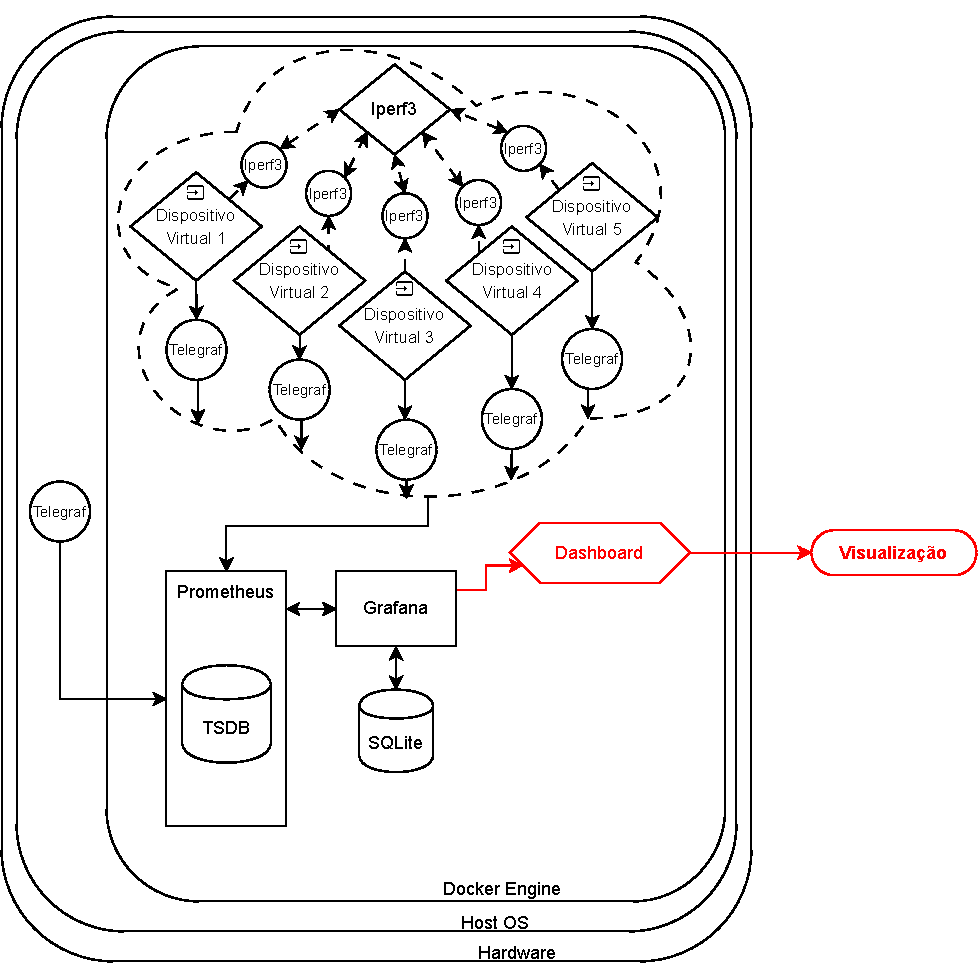
\includegraphics[width=\textwidth]{Imagens/chap03/by-blocks/dashboard_diagram.pdf}
\caption{Visualização.}
\label{fig:DiagramaVisualizacao}
\end{figure}

\begin{figure}[H]
\centering
\color{red}
\setlength{\abovecaptionskip}{-20pt}
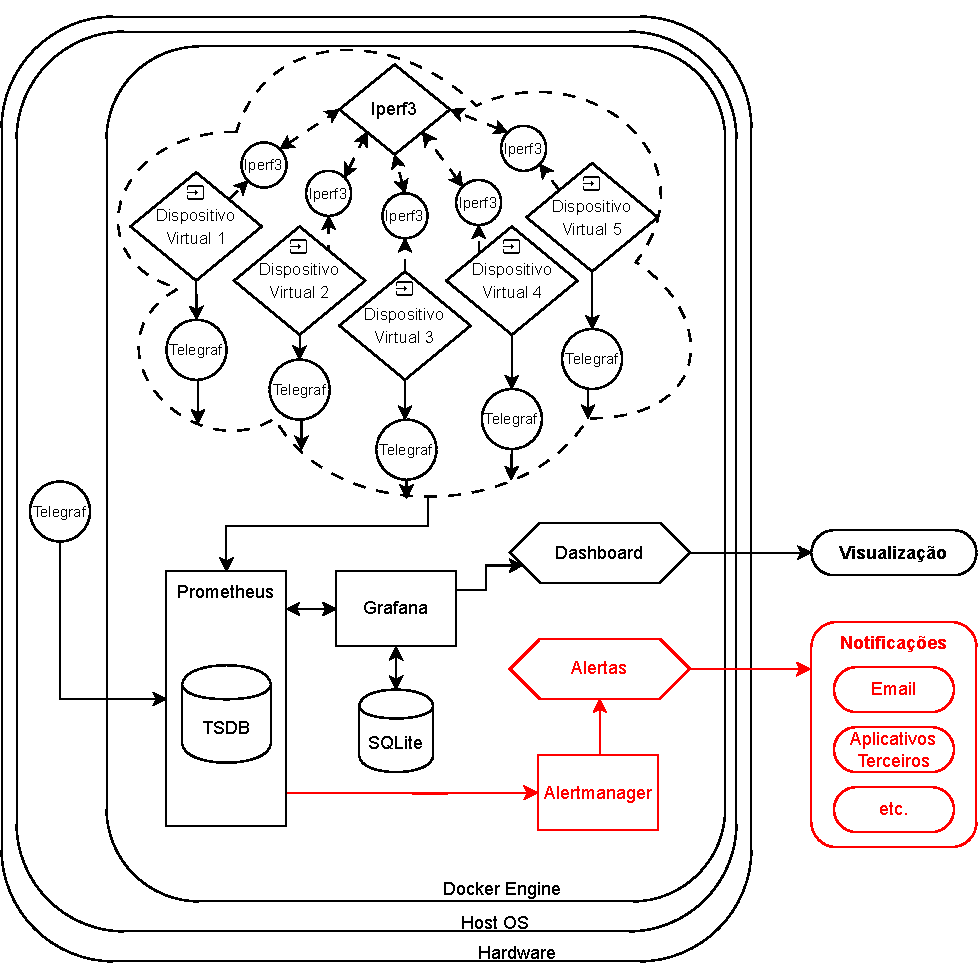
\includegraphics[width=\textwidth]{Imagens/chap03/by-blocks/alerts_diagram.pdf}
\caption{Notificações e Arquitetura Final.}
\label{fig:DiagramaAlertas}
\end{figure}


\begin{figure}[H]
\centering
\color{red}
\setlength{\abovecaptionskip}{-20pt}
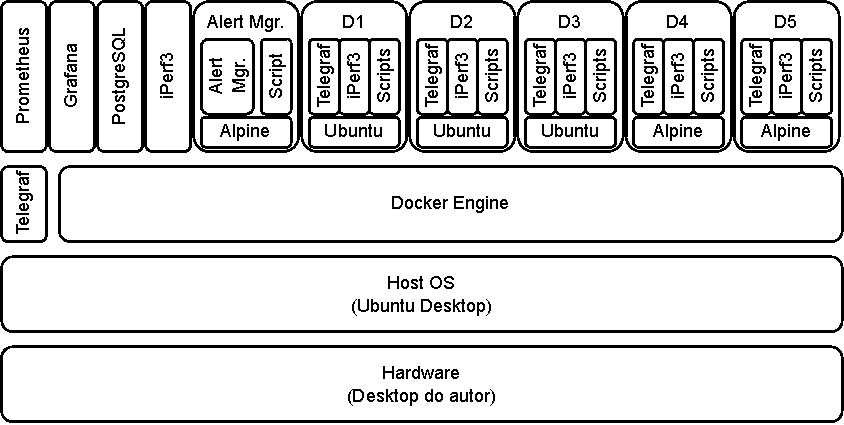
\includegraphics[width=\textwidth]{Imagens/chap04/final_stack.pdf}
\caption{\foreign{Stack} final.}
\label{fig:StackFinal}
\end{figure}

